\documentclass [11pt,twoside]{article}
\usepackage[utf8]{inputenc}
\usepackage[T1]{fontenc}

%Page margins, header and footer positions
\usepackage{geometry}
 \geometry{
 a4paper,
 total={210mm,297mm},
 left=25mm,
 right=25mm,
 top=30mm,
 bottom=25mm,
 headsep=7mm}

\interfootnotelinepenalty=10000

%To display filling dots in the TOC for all entries
\usepackage[titles]{tocloft}
\renewcommand{\cftsecleader}{\cftdotfill{\cftdotsep}}

%Define new header and footer style
\usepackage{fancyhdr}

\pagestyle{fancy}
\fancyhf{}
\lhead{\color{Gray}{\small{CLup project by Francesco Attorre, Thomas Jean Bernard Bonenfant, Veronica Cardigliano}}}
\lfoot{\textcolor{Gray}{\small{Copyright © 2021, Francesco Attorre, Thomas Jean Bernard Bonenfant, Veronica Cardigliano – All rights reserved}}}
\rfoot{\textcolor{Gray}{\thepage}}
\renewcommand{\headrulewidth}{0pt}

%PACKAGES
\usepackage{wasysym}
\usepackage{pifont}

\newcommand{\supported}{\ding{52}\xspace}
\newcommand{\unsupported}{\ding{55}\xspace}
\newcommand{\partsupported}{\textcolor{black!40}{\ding{52}}\xspace}
\newcommand{\lowsupported}{\textcolor{black!20}{\ding{52}}\xspace}
\newcommand{\unknowsupported}{\textbf{?}\xspace}

%Font: Times
\usepackage{times}
%Change monospaced font
\renewcommand{\ttdefault}{lmtt}

%tables
\usepackage{tabu}
\usepackage{tabularx}
\usepackage{ltablex}
\usepackage{longtable}
\usepackage{float} % To allow the use of H modifier in long tables

%landscape mode
\usepackage{pdflscape}
\usepackage{rotating}
\usepackage{caption}

%make landscape mode be sensitive to even and odd pages
%start
\def\myrotate{\ifodd\c@page\else-\fi 90}
\makeatletter
\global\let\orig@begin@landscape=\landscape%
\global\let\orig@end@landscape=\endlandscape%
\gdef\@true{1}
\gdef\@false{0}
\gdef\landscape{%
    \global\let\within@landscape=\@true%
    \orig@begin@landscape%
}%
\gdef\endlandscape{%
    \orig@end@landscape%
    \global\let\within@landscape=\@false%
}%
\@ifpackageloaded{pdflscape}{%
    \gdef\pdf@landscape@rotate{\PLS@Rotate}%
}{
    \gdef\pdf@landscape@rotate#1{}%
}
\let\latex@outputpage\@outputpage
\def\@outputpage{
    \ifx\within@landscape\@true%
        \if@twoside%
            \ifodd\c@page%
                \gdef\LS@rot{\setbox\@outputbox\vbox{%
                    \pdf@landscape@rotate{-90}%
                    \hbox{\rotatebox{90}{\hbox{\rotatebox{180}{\box\@outputbox}}}}}%
                }%
            \else%
                \gdef\LS@rot{\setbox\@outputbox\vbox{%
                    \pdf@landscape@rotate{+90}%
                    \hbox{\rotatebox{90}{\hbox{\rotatebox{0}{\box\@outputbox}}}}}%
                }%
            \fi%
        \else%
            \gdef\LS@rot{\setbox\@outputbox\vbox{%
                \pdf@landscape@rotate{+90}%
                \hbox{\rotatebox{90}{\hbox{\rotatebox{0}{\box\@outputbox}}}}}%
            }%
        \fi%
    \fi%
    \latex@outputpage%
}
\makeatother
%end

%graphics
\usepackage{graphicx}
\usepackage[dvipsnames, table]{xcolor}

%References
%\usepackage{xpatch}
%\usepackage[backend=biber, style=numeric, citestyle=numeric, sorting=none]{biblatex}
%\addbibresource{main.bib}

%Other
\usepackage{ifthen}
\usepackage{xspace}
\usepackage{enumitem}
\usepackage{amssymb}
\usepackage[pdftex, colorlinks]{hyperref}
\newcommand{\comment}[1]{{\color{Red}$\blacktriangleright$ Comment: #1 $\blacktriangleleft$}}


% Some utilities\ldots
\usepackage{soul}
\usepackage{tikz}

\usetikzlibrary{calc}
\usetikzlibrary{decorations.pathmorphing}


\makeatletter

\newcommand{\defhighlighter}[3][]{%
  \tikzset{every highlighter/.style={color=#2, fill opacity=#3, #1}}%
}

\defhighlighter{yellow}{.5}

\newcommand{\highlight@DoHighlight}{
  \fill [ decoration = {random steps, amplitude=1pt, segment length=15pt}
        , outer sep = -15pt, inner sep = 0pt, decorate
       , every highlighter, this highlighter ]
        ($(begin highlight)+(0,8pt)$) rectangle ($(end highlight)+(0,-3pt)$) ;
}

\newcommand{\highlight@BeginHighlight}{
  \coordinate (begin highlight) at (0,0) ;
}

\newcommand{\highlight@EndHighlight}{
  \coordinate (end highlight) at (0,0) ;
}

\newdimen\highlight@previous
\newdimen\highlight@current

\DeclareRobustCommand*\highlight[1][]{%
  \tikzset{this highlighter/.style={#1}}%
  \SOUL@setup
  %
  \def\SOUL@preamble{%
    \begin{tikzpicture}[overlay, remember picture]
      \highlight@BeginHighlight
      \highlight@EndHighlight
    \end{tikzpicture}%
  }%
  %
  \def\SOUL@postamble{%
    \begin{tikzpicture}[overlay, remember picture]
      \highlight@EndHighlight
      \highlight@DoHighlight
    \end{tikzpicture}%
  }%
  %
  \def\SOUL@everyhyphen{%
    \discretionary{%
      \SOUL@setkern\SOUL@hyphkern
      \SOUL@sethyphenchar
      \tikz[overlay, remember picture] \highlight@EndHighlight ;%
    }{%
    }{%
      \SOUL@setkern\SOUL@charkern
    }%
  }%
  %
  \def\SOUL@everyexhyphen##1{%
    \SOUL@setkern\SOUL@hyphkern
    \hbox{##1}%
    \discretionary{%
      \tikz[overlay, remember picture] \highlight@EndHighlight ;%
    }{%
    }{%
      \SOUL@setkern\SOUL@charkern
    }%
  }%
  %
  \def\SOUL@everysyllable{%
    \begin{tikzpicture}[overlay, remember picture]
      \path let \p0 = (begin highlight), \p1 = (0,0) in \pgfextra
        \global\highlight@previous=\y0
        \global\highlight@current =\y1
      \endpgfextra (0,0) ;
      \ifdim\highlight@current < \highlight@previous
        \highlight@DoHighlight
        \highlight@BeginHighlight
      \fi
    \end{tikzpicture}%
    \the\SOUL@syllable
    \tikz[overlay, remember picture] \highlight@EndHighlight ;%
  }%
  \SOUL@
}

\makeatother

% Common abbrev. are set as commands to ensure proper spacing after the dot
\RequirePackage{xspace}
\newcommand{\ie}{i.e.\@\xspace}
\newcommand{\aka}{a.k.a.\@\xspace}
\newcommand{\Ie}{I.e.\@\xspace}
\newcommand{\cf}{cf.\@\xspace}
\newcommand{\Cf}{Cf.\@\xspace}
\newcommand{\eg}{e.g.\@\xspace}
\newcommand{\Eg}{E.g.\@\xspace}
\newcommand{\etal}{et al.\@\xspace}
\newcommand{\etc}{etc.\@\xspace}
\newcommand{\wrt}{w.r.t.\@\xspace}
\newcommand{\Wrt}{W.r.t.\@\xspace}



\date{}

\usepackage{graphicx}
\graphicspath{ {./images/} }

\usepackage[dvipsnames]{xcolor}
\usepackage{listings}
\usepackage{alloy-style}

\usepackage{multirow}

\begin{document}

%TITLE PAGE

\begin{titlepage}


%LOGO

\begin{center}
    
\includegraphics[height=5cm]{Logo_Polimi}\\
    \vspace{7cm}
      \begin{huge}
        \textbf{CLup - Customer Line Up}\\
      \end{huge}
      \vspace{0.3cm}
      \begin{large}
        \textit{Software Engineering 2 Project 2020/21}\\
      \end{large}
      
      \vfill
      \begin{author}
        \textbf{\Large Authors}\\
        \begin{itemize}
          \item Francesco Attorre - \textit{10618456}\\
          \item Thomas Jean Bernard Bonenfant - \textit{10597564}\\
          \item Veronica Cardigliano - \textit{10627267}\\
        \end{itemize}
      \end{author}

    \end{center}
  
  \end{titlepage}

%Define deliverable specific info
%Replace cell contents where needed
\begin{table}[h!]
\begin{tabu} to \textwidth { X[0.3,r,p] X[0.7,l,p] }
\hline

\textbf{Deliverable:} & DD\\
\textbf{Title:} & Design Document \\
\textbf{Authors:} & Francesco Attorre, Thomas Jean Bernard Bonenfant, Veronica Cardigliano \\
\textbf{Version:} & 1.0 \\ 
\textbf{Date:} & 10-January-2021 \\
\textbf{Download page:} & https://github.com/FrancescoAttorre/softeng2-attorre-bonenfant-cardigliano \\
\textbf{Copyright:} & Copyright © 2021, Francesco Attorre, Thomas Jean Bernard Bonenfant, Veronica Cardigliano - All rights reserved \\
\hline
\end{tabu}
\end{table}

\setcounter{page}{2}


%------------------------------------------------------------------------------------------------------------------------------------------------
%Table Of Contents
\newpage

\addcontentsline{toc}{section}{Table of Contents}
\hypersetup{linkcolor = black}
\tableofcontents

\newpage
%\addcontentsline{toc}{section}{List of Figures}
%\listoffigures
%\addcontentsline{toc}{section}{List of Tables}
%\listoftables

%------------------------------------------------------------------------------------------------------------------------------------------------
%Introduction
\clearpage
{\color{Cerulean}{\section{Introduction}}}
\label{sect:introduction}
\renewcommand{\thesubsection}{\Alph{subsection}}
\subsection{Introduction}
The goal of this document (I\&T: Implementation and Testing) is to describe the structure of the implementation of CLup, together with the main frameworks adopted for its development. It also includes informations about how the testing plan. This document is preceded by the RASD (Requirements Analysis and Specification Document) and DD (Design Document) documents. In particular, the implementation has been driven by the decisions made in the Design Document, about the main components, interfaces and architectural patterns to exploit, and also implementation, integration and testing plans.
\subsection{Scope}
This document illustrates how the implementation of CLup system has been carried on. CLup is an application which aims to avoid the occurrence of crowds in a period of global pandemic. To achieve this goal, it allows customers to queue before entering a building without creating long physical queues in front of it, or to book a visit to access a building, through an application. CLup will allow people to save time and be safer, managing both the accesses of people who use the application directly, and of people who go physically to the store, using store managers as intermediaries. CLup can be accessed by activities, which will register their buildings giving all the necessary information, by store managers who manage the entrances to the building they're related to, and by customers. Booking a visit, customers can also decide how much time they want spend in the building and, optionally, which specific departments they want to visit, in order to allow a greater number of people to enter when possible.
\newpage

%------------------------------------------------------------------------------------------------------------------------------------------------
%Overall Description
\clearpage
{\color{Cerulean}{\section{Architectural Design}}}
\label{sect:architecturalDesign}
%Product Perspective
\subsection{Overview: High-level components and their interaction}

The architectural style chosen to develop the system is a three layer architecture, with a layer of Presentation, one of Business logic/Application and one of Data. This style has been chosen since it allows an easy decoupling of logic and data and of logic and presentation. The presentation level is the one which handles interactions with users, with the interfaces to communicate with them.
The Business logic consists in the functions provided to the users. Moreover, this layer handles the communication between the other two layers. The data access layer, instead, manages the access to the database both for storing and retrieving data for the other layers. The hardware architecture chosen is the three-tier one. An advantage of this architecture is that the client tier doesn't communicate directly with the DBMS, so the middle tier guarantee a major level of security. Moreover, in this way the connection with the DBMS will be persistent and consequently less expensive. These application layers are divided into three physical dedicated machines. A mobile device/pc, basing on the type of user, that is a personal computer for the activities and a mobile phone for customers and store managers, is used to interface with the user. The Business logic, instead, is the application server which communicates with the DatabaseServer.

\subsection{Component view}
\begin{figure}[H]
	\centering
	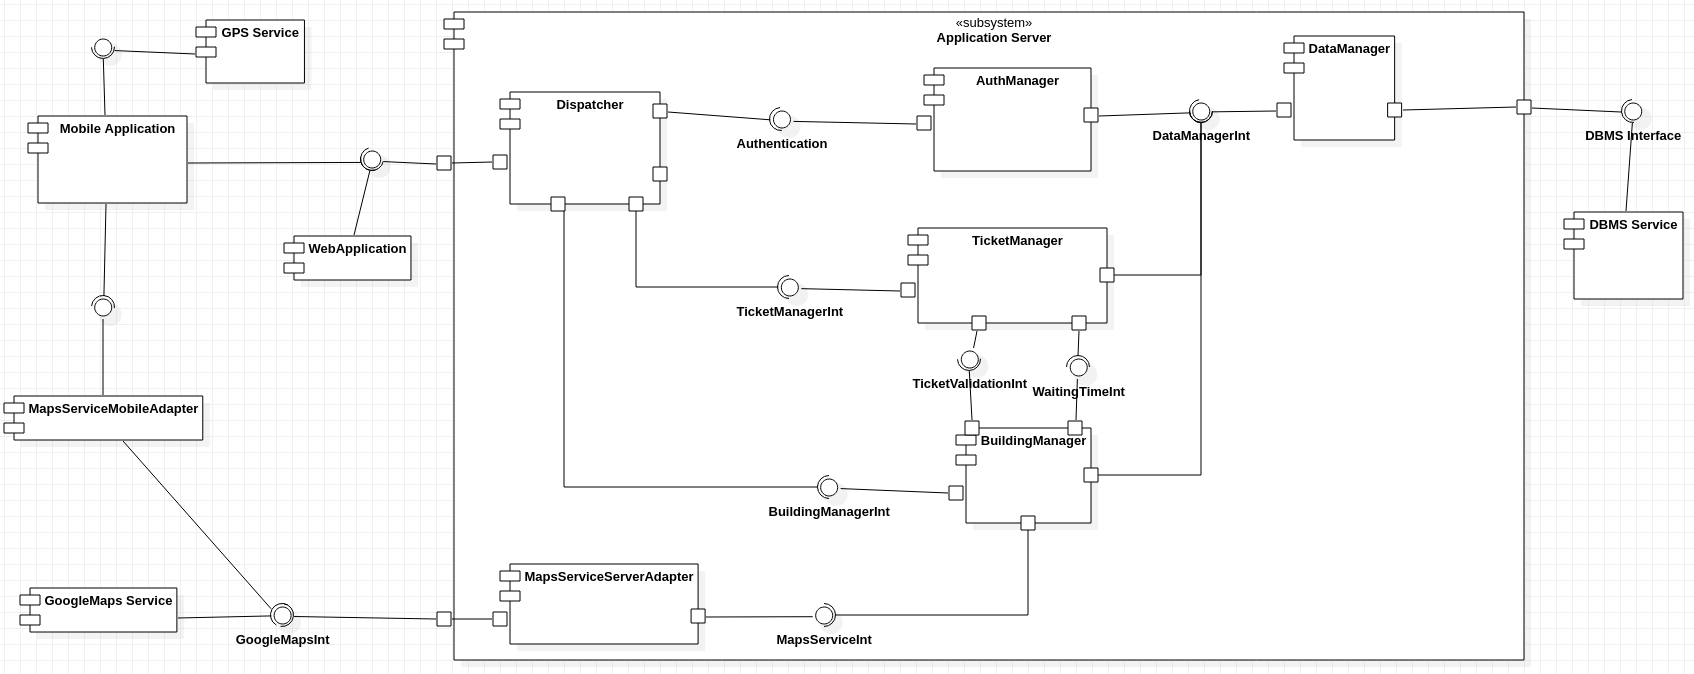
\includegraphics[width=1\textwidth]{/Diagrams/ComponentDiagram}
	\caption{Component Diagram}
\end{figure}



\textbf{TicketManager}\\
This component provides services to deliver new tickets, change their state and communicates with BuildingManager to associate them with a Building.\\
\textbf{AuthManager}\\
This component offers services to authenticate users and deliver them tokens that authorize to use the other services. The dispatcher component will ask the Auth Manager to check the token validity before forwarding requests to other Components.\\
\textbf{BuildingManager}\\
Provides services to add buildings to the system, track the number of people in specific buildings, append and pop line up tickets from queues and add booking tickets to a building.\\
\textbf{RegistrationService}\\
Allows UnregisteredAppCustomers and Activities to register to CLup through its service.\\
\textbf{GoogleMapsService}\\
External service component that provides web mapping. Used to locate Buildings nearby.\\
\textbf{Dispatcher}\\
This component manages the requests received from MobileApp and Web Server components and redirects each one to the correct component able to handle it.\\
\textbf{Mobile Application}\\
Acts as a Client sending requests to the Dispatcher component.
It is a fat client since it does contain Applicative logic.\\
\textbf{Web Application}\\
Web Client sending requests to the Dispatcher like the Mobile Application. It will be thinner than the Mobile Application taking part only at the Presentation Level since it does not contain any Applicative logic.\\
\textbf{DataManager}\\
Manages data structures and objects to persist to the database.\\
\textbf{DBMS Service}\\
Represents the DBMS and the service he offers. It communicates with the DataManager\\
\textbf{GPS Service}\\
Positioning system used to locate a device.\\
\textbf{MapsServiceMobileAdapter}\\
Adapter that offers to the MobileApplication component an interface for using Mapping services. Useful if the external Mapping service changes the Mobile Application will always used the same interface.\\
\textbf{MapsServiceServerAdapter}\\
Like previous adapter but for the BuildingManager component. Having 2 different Adapters offers the possibility to use different Mapping services for MobileApplication and BuildingManager 


\subsection{Deployment view}
\begin{figure}[H]
	\centering
	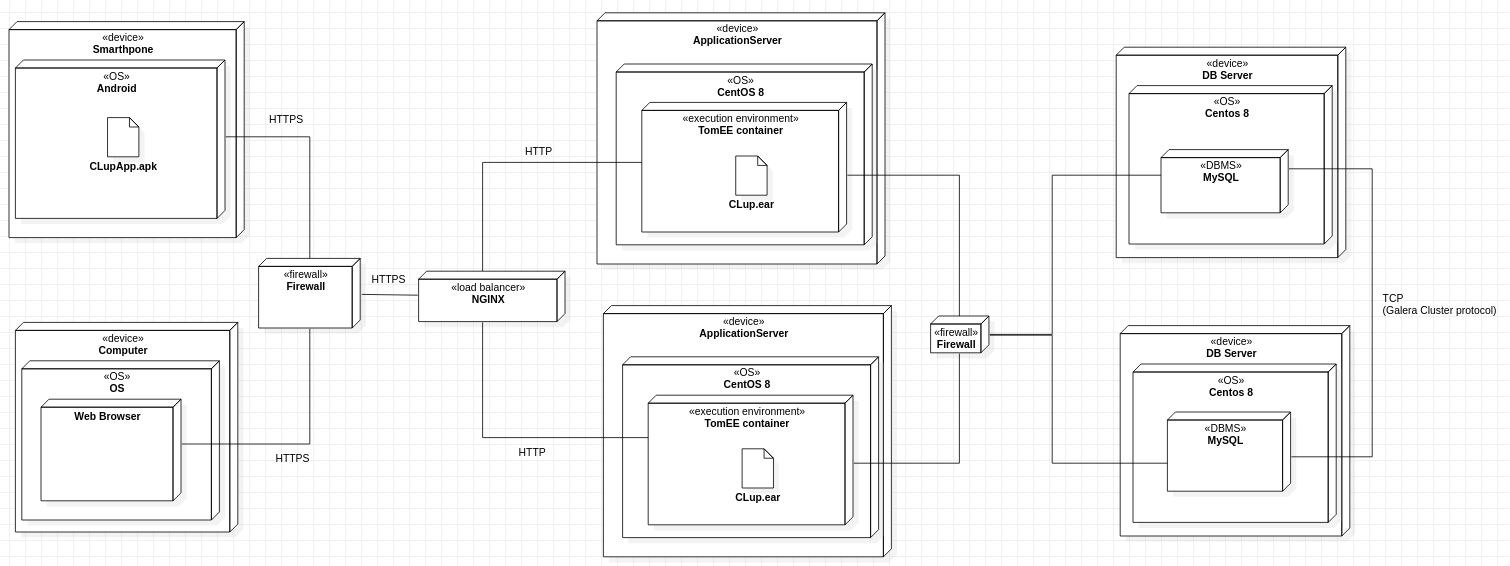
\includegraphics[width=1.1\textwidth]{/Diagrams/DeploymentDiagram}
	\caption{Deployment Diagram}
\end{figure}

This diagram shows the overall deployment architecture. Here is a description of every element:\\
\begin{itemize}
    \item \textbf{Smartphone}: Device used by AppCustomers and StoreManagers. It will have to contain the CLup App executable in order to use the system.
    
    \item \textbf{Computer}: Device used by Activities in order to use the WebApp.
    
    \item \textbf{Firewall}: Provides safety access to the internal network of the system as part of the safety of the system against external attacks.
    
    \item \textbf{Nginx}: Nginx server used to balance the load on the multiple Application servers. It is responsible to establish an encrypted connection with the clients through Transport Layer Security (TLS). From this point on the connection will be unencrypted as we consider the internal network as secure.
    
    \item \textbf{ApplicationServer}: Contains most of the Application Logic. Because of the stateless behavior of the server side logic Application Servers can be easily added to scale out and maintain high availability and reliability. The CLup.ear artifact is the implementation of the ApplicationServer subsystem found in the Component Diagram.
    
    \item \textbf{DB Server}: It implements the DBMS Service in the Component Diagram. It is part of a Galera Cluster, a synchronous replication solution, transparent to the Application Servers to improve availability and performance of the DBMS Service. The Cluster will be deployed in a distributed load balancing configuration: each Application server will have a JDBC connector configured for load balancing; this avoids to have between the Application Servers and the Database Servers a separated load balancer that could be a single point of failure (if an ulterior backup load balancer is not added) and a potential bottleneck.

\end{itemize}



\subsection{Runtime view}
Here are proposed sequence diagrams in order to describe the way components interact with each other to accomplish specific tasks.\\

\begin{center} 
Premise\\
\end{center}
It’s not explicitly stated in every sequence diagram that a token checking is performed for every request done from Clients to the Server. The Dispatcher, before processing the request just received, will perform on AuthServer a token validity check, which comprises a verification on the funcionality that a Client can request on the Server. \\ 
Instead the identification action performed in some diagrams has the task to retrieve the User information, usually an identifier.\\

\newpage
\subsubsection{Authentication Sequence Diagram}
\textit{Two different authentication procedures can occur, the first is an authentication on a RegisteredAppCustomer, instead a daily access to CLup services can be requested by UnregisteredAppCustomer.\\}
\textbf{Description\\}
Both of the following process lead to gaining a token, that is a temporary access key for Server functionalities. The second one is Daily in the sense that every operation on server would stay for at most one day.\\
account based - an authentication request is made by the MobileApplication, after correctly forwarding this request to AuthManager an account check is done. If the user exists and has no token already associated with its account, then a new one will be created. MobileApplication receives a response containing his token. \\
daily - a daily authentication request is made by the MobileApplication, after correctly forwarding this request to AuthManager an access check is done. If the client can get a token in order to access server basic functions a new association between a specific MoibleApplication and a new token is made, else a negative response is sent back to the client. \\

\begin{figure}[H]
 \centering
 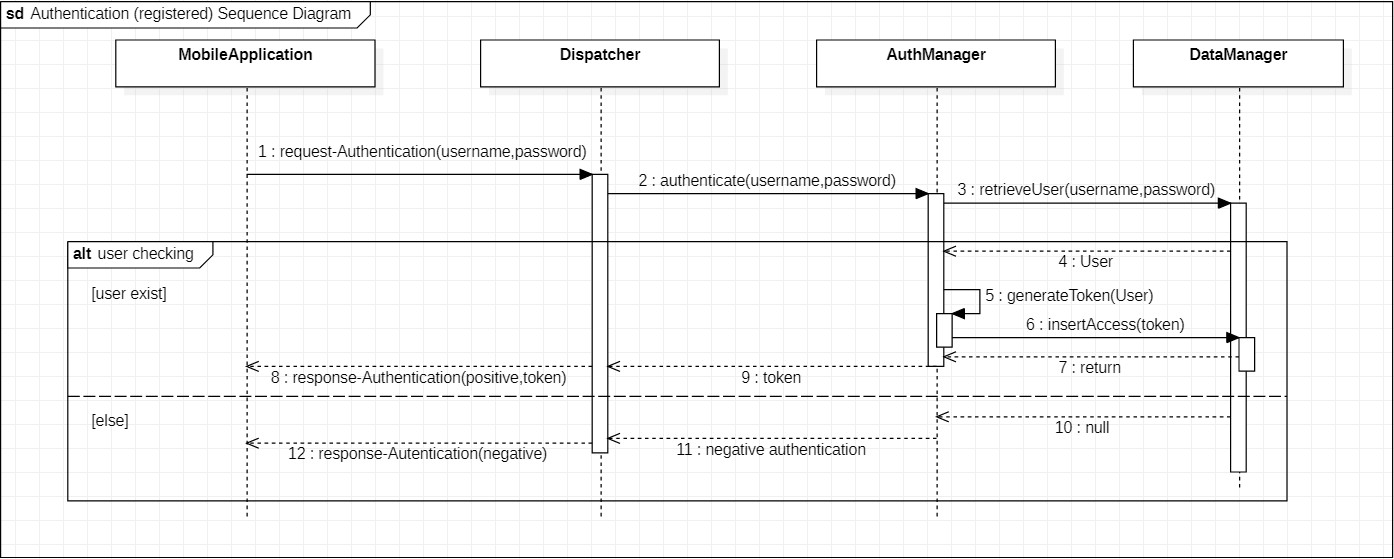
\includegraphics[width=\textwidth]{Authentication (registered) Sequence Diagram}
 \caption{ Authentication (registered) Sequence Diagram}
 \end{figure}

\newpage
\begin{figure}[H]
 \centering
 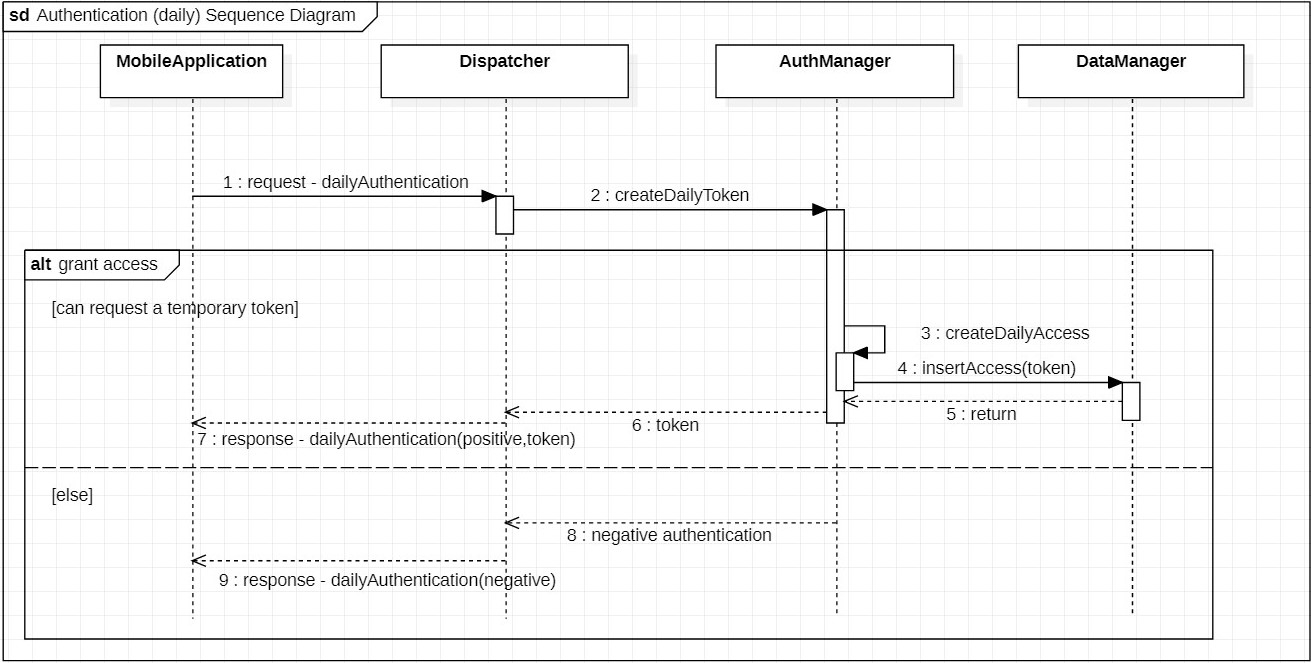
\includegraphics[width=\textwidth]{Authentication (daily) Sequence Diagram}
 \caption{Authentication (daily) Sequence Diagram}
 \end{figure}

\newpage
\subsubsection{ Acquire a LineUpDigitalTicket Sequence Diagram}
\textit{This diagram explains how an AppCustomer can acquire a LineUpDigitalTicket.\\}
\textbf{Description\\}
MobileApplication retrieves a position (manually or through GPS) and sends a request in order to receive a list of buildings from which one would be selected. Building retrieval is effectively done by the DataManager. Whereas the MapsServiceAdapter (communication with a maps API) provides to BuildingManager useful information to correctly pick only reachable buildings.\\
Once the building is selected, MobileApplication sends another request in order to gain a ticket. An identification is performed on AuthManager to correctly retrieve the UserID (associated to the token) needed in ticket acquisition. Afterwards, to complete the process,if the building has at least one void space the ticket state is setted to Valid, else the ticket is inserted in queue.
If ticket insertion goes wrong a negative acknowledgment is sent back.\\
Note that only after a Discovery request from the MobileApplication, this ticket will produce a notification (as described in Discovery diagram).\\
\textbf{Variant\\}
MobileApplication ticket request performed by a StoreManager works equally, but building list is not requested because of it is constrained by the one for which StoreManager is signed in. \\

\begin{figure}[H]
 \centering
 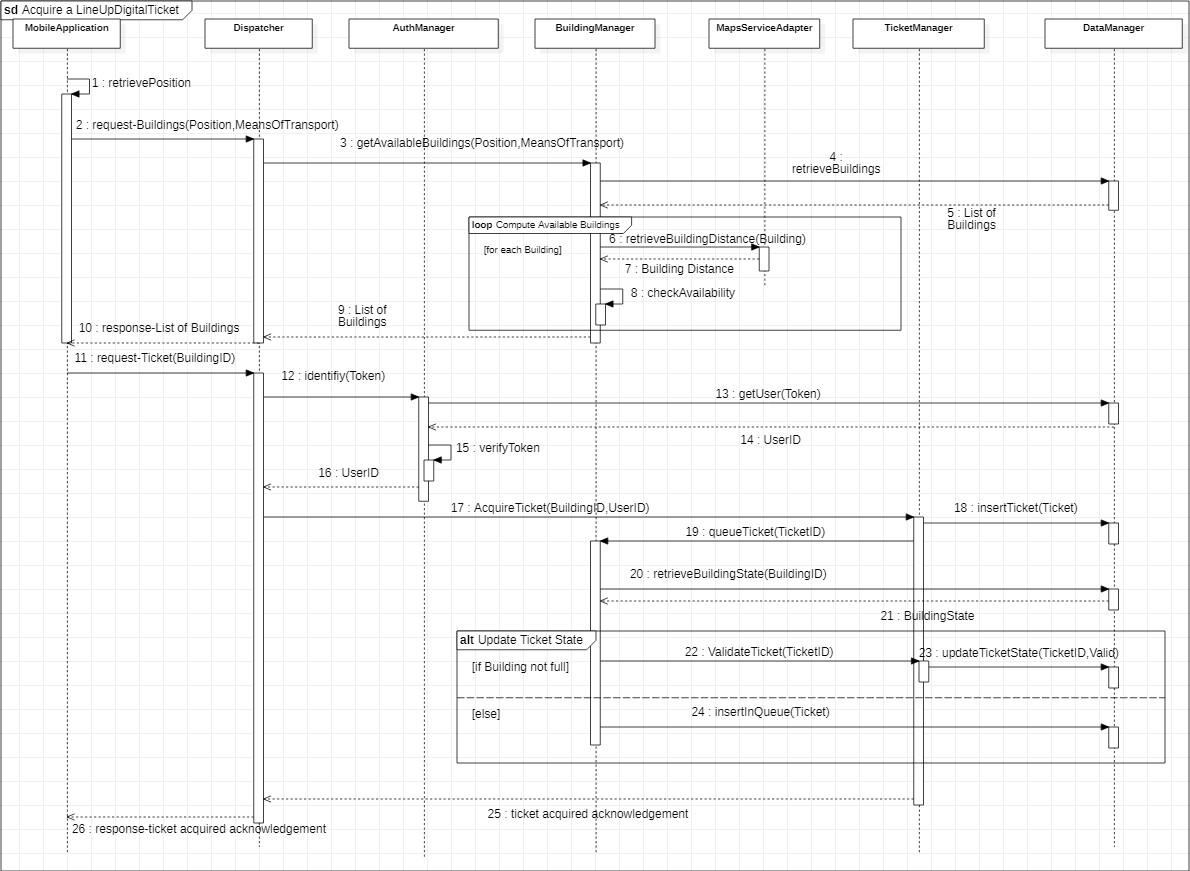
\includegraphics[width=\textwidth]{Acquire a LineUpDigitalTicket Sequence Diagram}
 \caption{ Acquire a LineUpDigitalTicket Sequence Diagram}
 \end{figure}

\newpage
\subsubsection{Acquire a BookingDigitalTicket Sequence Diagram}
\textit{This diagram explains how a RegisteredAppCustomer can acquire a BookingDigitalTicket\\}
\textbf{Description\\}
MobileApplication retrieves a position (manually or through GPS) and sends a request with the purpose to receive a list of buildings from which one would be selected.
Building retrieval is effectively done by the DataManager. Whereas the MapsServiceAdapter (communicating with a maps API) provides BuildingManager useful information to correctly pick only reachable buildings.\\
Once the building is selected, MobileApplication sends another request in order to have a list of TimeSlots. Dispatcher forwards this request to the BuildingManager that primarily retrieves Building which capacity information is needed to compute TimeSlots availability for a specific date.\\
Lastly MobileApplication requests the Server to gain a ticket. An identification is performed on AuthManager to correctly retrieve the UserID (associated with the token) needed in ticket acquisition. Then a general check validity is performed by BuildingManager, non valid tickets will be not acquired. An acknowledgement is sent back to MobileApplication.

\begin{figure}[H]
 \centering
 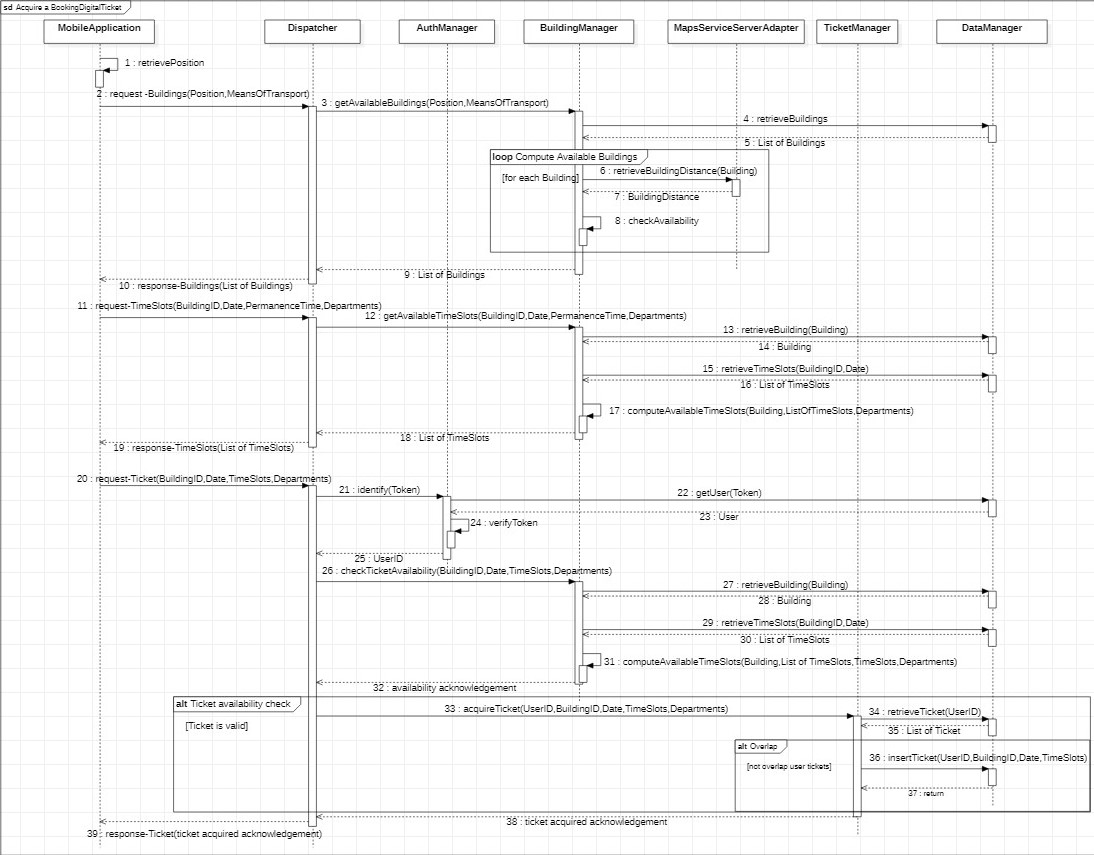
\includegraphics[width=\textwidth]{Acquire a BookingDigitalTicket Sequence Diagram}
 \caption{ Acquire a BookingDigitalTicket Sequence Diagram}
 \end{figure}

\newpage
\subsubsection{Discovery Sequence Diagram}
\textit{This diagram explains how an AppCustomer can be notified about when to start reaching a Building and about its ticket validity or a StoreManager when to inform validity of some PhysicalCustomers’s Tickets.\\}
\textbf{Description\\}
A Discovery request is a polling request made by a MobileApplication in order to receive updates about Tickets. The Dispatcher first identifies the User and then get updated waiting time estimation from TicketManager.\\
The waiting time computation process is made by means of a statistic (peculiar of each Building and kept up to date on every exit event) and the queue (which defines the ticket position) in the waiting time computation service. Waiting time depends also on exiting delays which would have a particular rounding.
Ticket and estimated waiting time for each ticket are sent back to Mobile Application, that will start checking all of them.\\
For AppCustomer a notification will be received based on the actual position and on ticket estimated waiting time, instead a StoreManager will check only for just validated tickets.
\\

\begin{figure}[H]
 \centering
 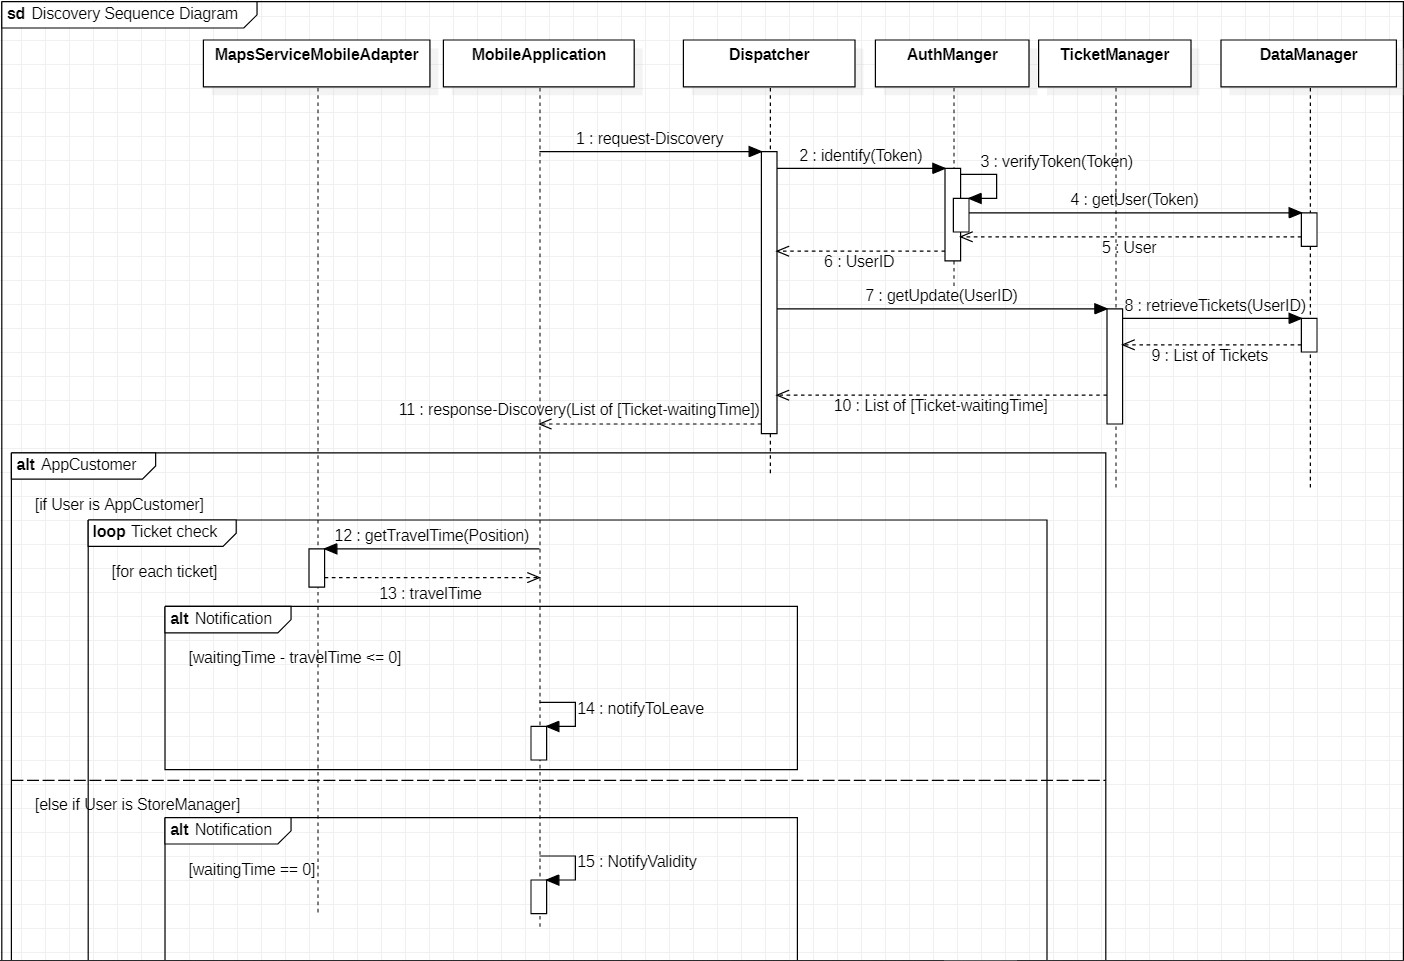
\includegraphics[width=\textwidth]{Discovery Sequence Diagram}
 \caption{ Discovery Sequence Diagram }
 \end{figure}

\newpage
\subsubsection{Customer Exit Building Sequence Diagram}
\textit{This diagram explains how a StoreManager can notify CLup about a Customer left the Building.\\}
\textbf{Description\\}
MobileApplication exit request is sent to Dispatcher that identify User(StoreManager associated with the Building for which he is signed up for) then the request is forwarded to BuildingManager.\\
It will keep up to date statistic (means of delta customer leave) and last exit time for that specific buildin, the nthe validation process will start. Queue is retrieved from DataManager and the next ticket in queue (if there is one) will be validated. An acknowledge for successful processing is received by Dispatcher and then MobileApplication.\\

\begin{figure}[H]
 \centering
 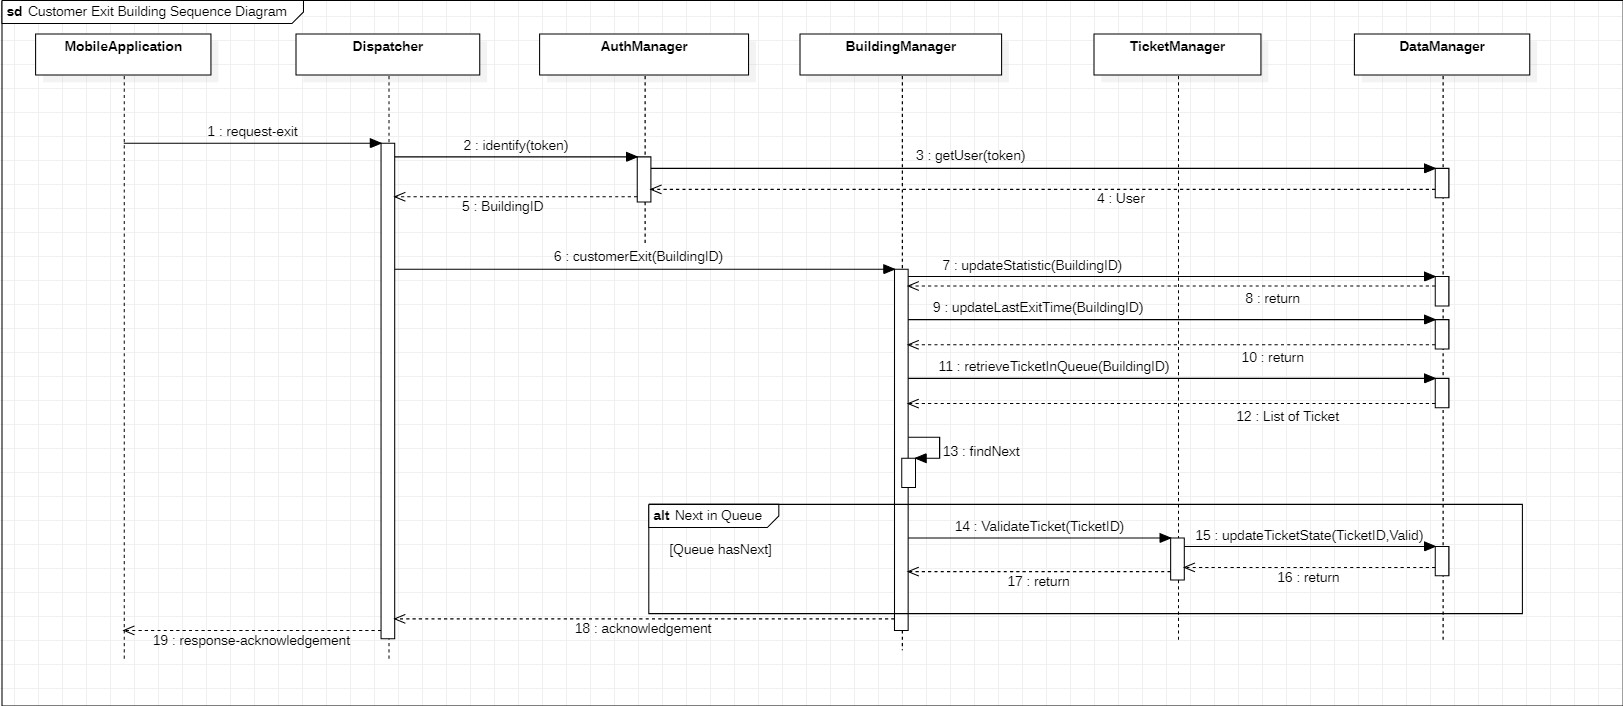
\includegraphics[width=\textwidth]{Customer Exit Building Sequence Diagram}
 \caption{ Customer Exit Building Sequence Diagram }
 \end{figure}

\newpage
\subsubsection{Activity Insert Building Sequence Diagram}
\textit{This diagram explains how an Activity can insert a new Building in CLup.\\}
\textbf{Description\\}
WebApplication requests to insert a building providing some parameters, and optionally departments with surplus capacity. Dispatcher receives the request, it firstly identifies the user (that should correspond to an Activity) and then forward the insertion request to BuildingManager, that in order to correctly check if the building can be inserted,it retrieves a list of all buildings and the location,through the MapsServiceServerAdapter, given by the address. At this point if the Building is valid it is persisted. An acknowledgement is sent back to WebApplication.\\

\begin{figure}[H]
 \centering
 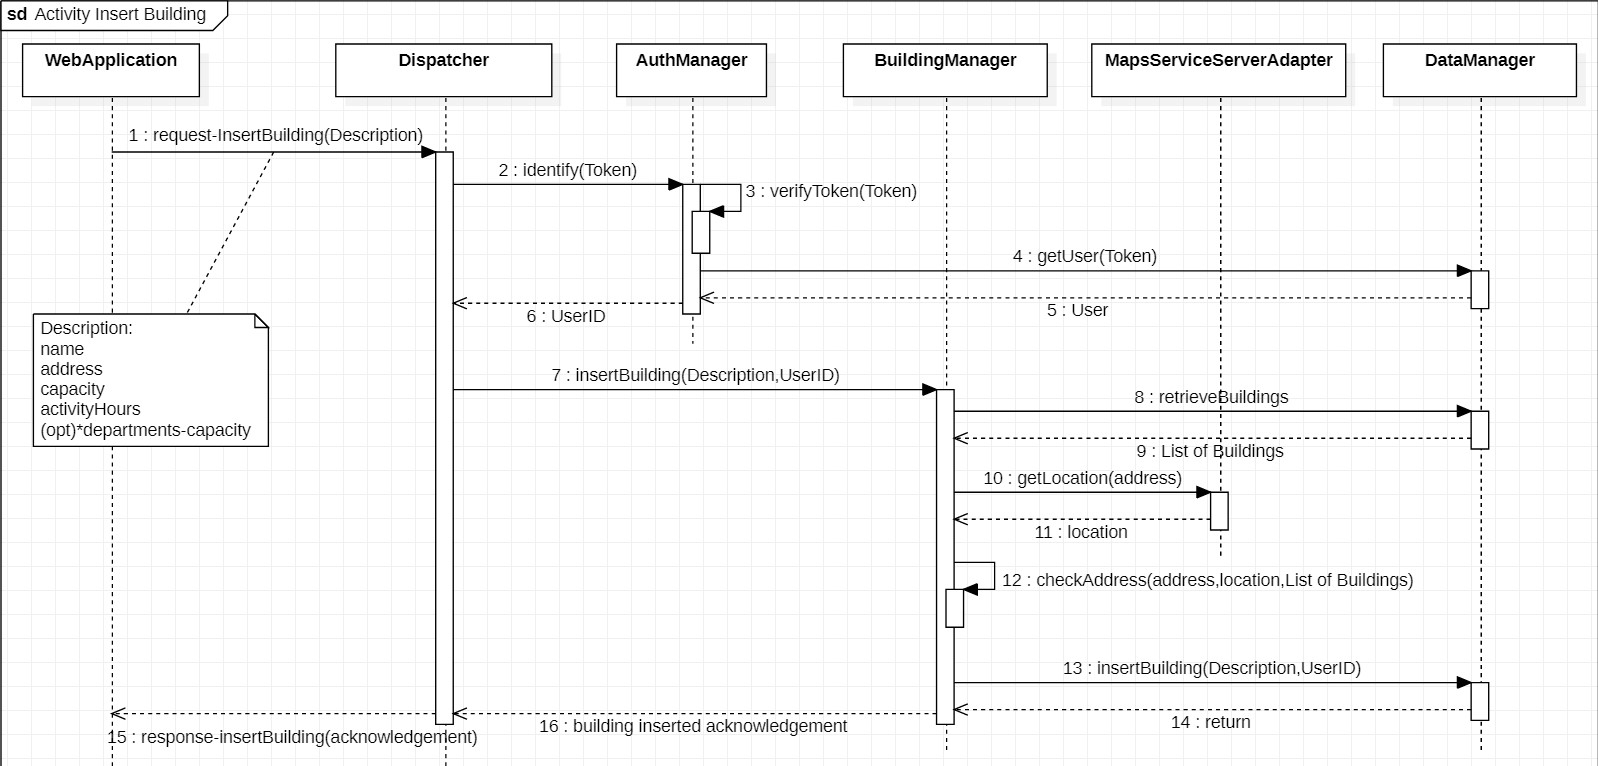
\includegraphics[width=\textwidth]{Activity Insert Building Sequence Diagram}
 \caption{ Activity Insert Building Sequence Diagram }
 \end{figure}

\newpage
\subsection{Component Interfaces}
The following diagram shows all the component interfaces already exploited in the sequence diagrams together with the dependencies between the various components. 
\newpage
\subsection{Selected architectural styles and patterns}
The architectural style selected is a three-tier client-server architecture, in order to have a good decoupling of logic, data and presentation, increasing reusability, flexibility and scalability. Moreover, components in the application server have to be developed mainly with low coupling among modules in order to make the system more comprehensible and maintainable. About the components, they have been designed to maintain a stateless logic as much as possible, that is, they should not contain an internal state, but refer to the database to get the necessary information. This is important since instances of components can fail and nothing must go lost in this eventuality. In this context the scalability of the database is so important, and DataAccessManager will play a leading role. 
The protocol used to send requests is HTTP, which is a good choice to implement a RESTful architecture to meet the above objectives of having a stateless and low coupling system. Other advantages are that it would be cacheable and with a uniform interface.
To ensure a secure and reliable communication between client and server, HTTPS is used with TLS encryption.
Data are transmitted in JSON, which is one of the simplest and most easily customizable protocol. It is also easy readable and allows fast parsing.\\
Finally, we've decided to use some design patterns in order to exploit existing models to solve recurrent problems. This benefits the reusability and maintainability of the code, as well as making it easier for designers to understand how the system works. Below the patterns used: \\
\subsubsection{Model View Controller - MVC}
MVC is a widely used pattern, particularly suitable for the development of applications written in object-oriented programming languages such as java. MVC is based on three main roles which are: the Model that contains all the methods to access the data useful to the application, the View that visualizes the data contained in the model and deals with the interaction with users and the Controller which receives the commands of the user and executes them them modifying the other two components. In CLup, the Controller logic is in the Dispatcher component, the Model is represented by services offered by the other application server's components, plus the DBMSAccessService, instead the view is in the Mobile and Web Applications.\\
\subsubsection{Adapter pattern}
Adapter is a structural pattern that aims to match interfaces of different classes. The interface of the Adapter is interposed between the system and the Adaptee, that is the object to be adapted. In this way, whoever has to use a method of the Adaptee sees only an interface (or an abstract class) which would be implemented according to the component to be adapted. In the case of CLup, the components MapsServiceMobileAdapter and MapsServiceServerAdapter act as the adapter for the mobile application and the server, and GoogleMapsService is the component to be adapted. In this way, even assuming that the external service is changed, the internal system will not undergo any changes, since the new API will be handled by these components.\\
\subsubsection{Facade pattern}
Facade is also a structural pattern, which consists in a single class representing the entire subsystem. In the case of CLup, the Dispatcher takes all the requests from the client and then directs them to the specific component of the AppServer. The aim of this component is to mask the complexity of the entire subsystem, with which you can communicate via a simple interface.
\newpage
\subsection {Other design decisions}
\subsubsection{Thin Client}
Having most of the business logic on server side, our client can be defined thin, although there are small pieces of business logic also in the client side. In fact, the client has a MapsServiceMobileAdapter to access the external component in order to compute independently the travel time in a real time way, in case it has decided to activate the GPS services. An advantage of this choice is a lighter communication with the server, which is not constantly updated on the position of the client when not necessary. Also the control on when to notify the client to leave for the building is made client side, given such information about position and time to reach it, avoiding to overload the server.
Another advantage of having a thin client with a little of business logic is that, having an application which works mainly online, in any case it will always be connected to the server having the main logic, but even if the connection would be interrupted, some services encapsulated in the client will still remain available.
\subsubsection{Database}
...
\newpage


%------------------------------------------------------------------------------------------------------------------------------------------------
%Specific Requirements
\clearpage
{\color{Cerulean}{\section{User Interface Design}}}
\label{sect:userInterface}
\begin{figure}[H]
	\centering
	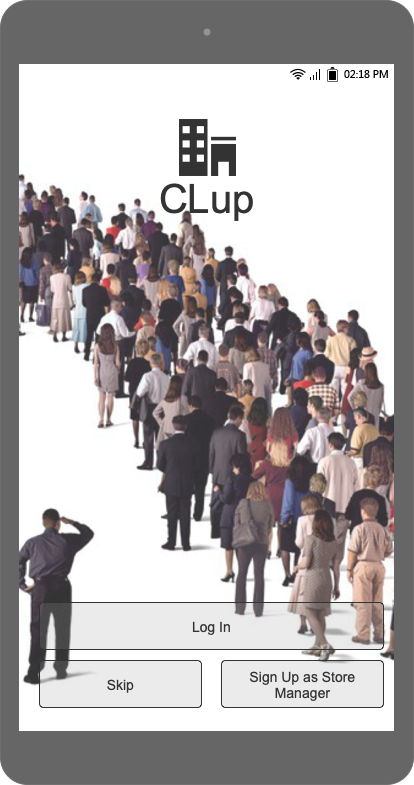
\includegraphics[width=0.33\textwidth]{/MockUps/Start}
	\caption{Starting page}
\end{figure}

\begin{figure}[H]
	\centering
	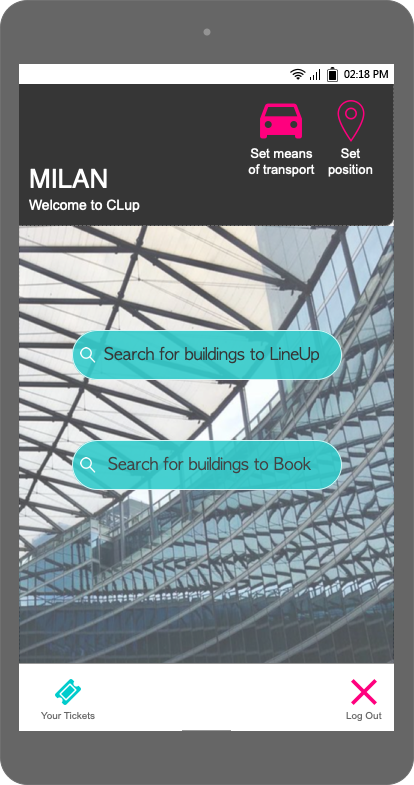
\includegraphics[width=0.33\textwidth]{/MockUps/HomePage}
	\caption{General home page of a registered customer}
\end{figure}

\newpage

\begin{figure}[H]
	\centering
	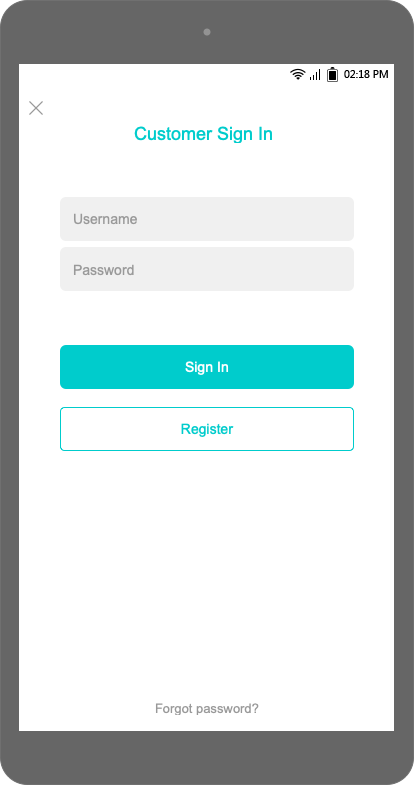
\includegraphics[width=0.33\textwidth]{/MockUps/SignIn}
	\caption{Interface for customers that want to sign in}
\end{figure}

\begin{figure}[H]
	\centering
	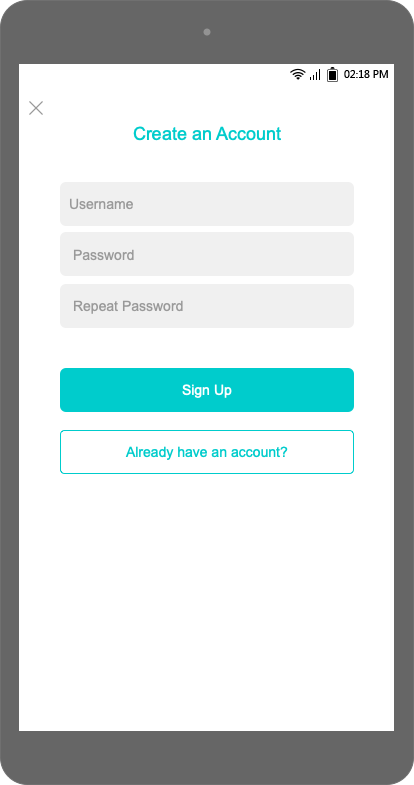
\includegraphics[width=0.33\textwidth]{/MockUps/SignUp}
	\caption{Interface for customers that want to register to CLup}
\end{figure}

\newpage

\begin{figure}[H]
	\centering
	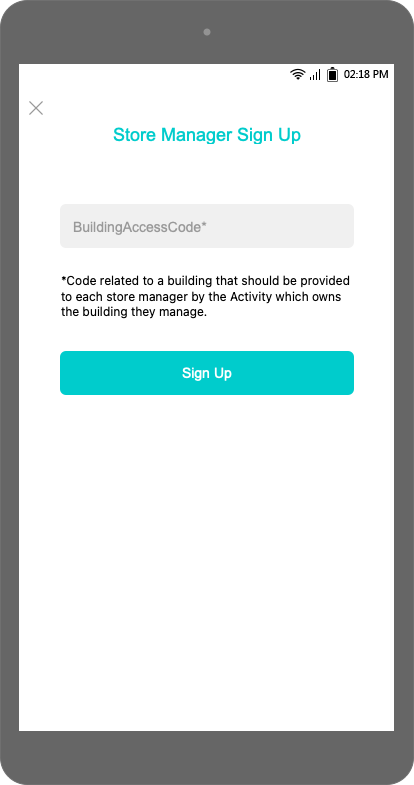
\includegraphics[width=0.33\textwidth]{/MockUps/StoreManagerSignUp}
	\caption{Interface for store managers to sign up}
\end{figure}

\begin{figure}[H]
	\centering
	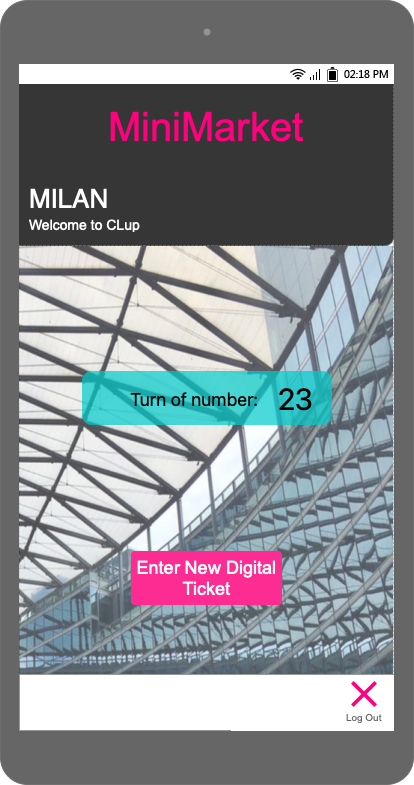
\includegraphics[width=0.33\textwidth]{/MockUps/StoreManagerHomePage}
	\caption{Home Page for store managers that have signed up}
\end{figure}

\newpage

\begin{figure}[H]
	\centering
	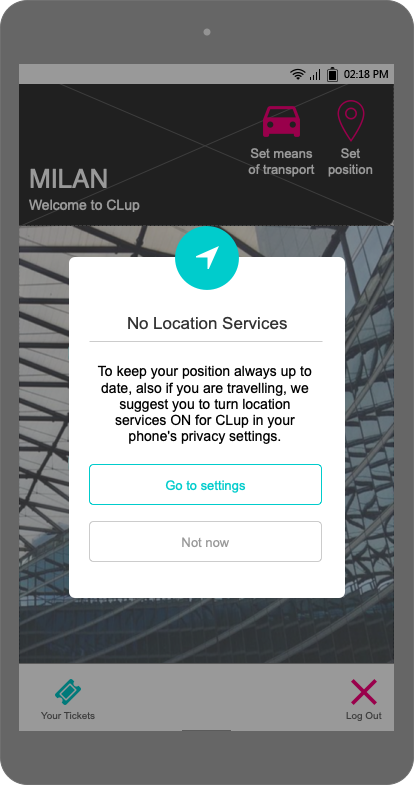
\includegraphics[width=0.33\textwidth]{/MockUps/SetGPS}
	\caption{Pop-up to activate GPS services}
\end{figure}

\begin{figure}[H]
	\centering
	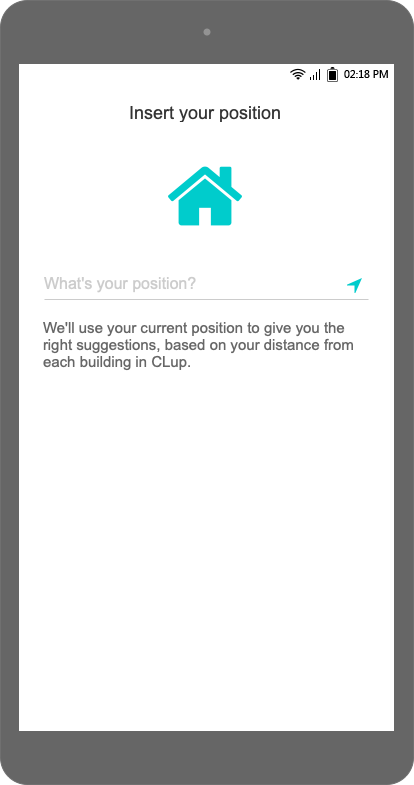
\includegraphics[width=0.33\textwidth]{/MockUps/SetLocation}
	\caption{Setting page to set a position manually}
\end{figure}

\newpage

\begin{figure}[H]
	\centering
	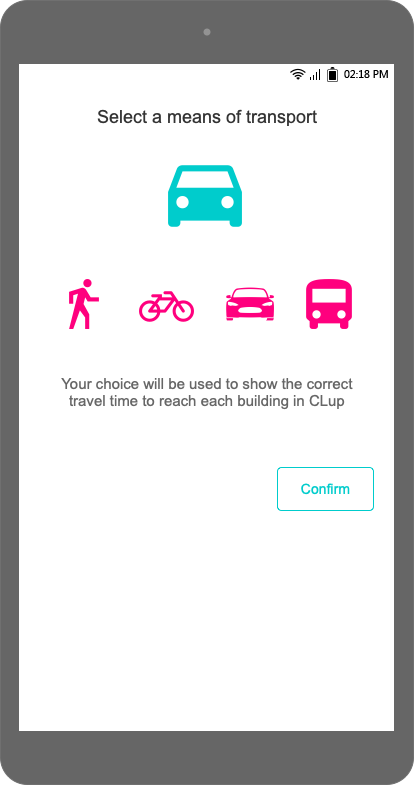
\includegraphics[width=0.33\textwidth]{/MockUps/SetMeansOfTransport}
	\caption{Setting page to choose a means of transport}
\end{figure}

\begin{figure}[H]
	\centering
	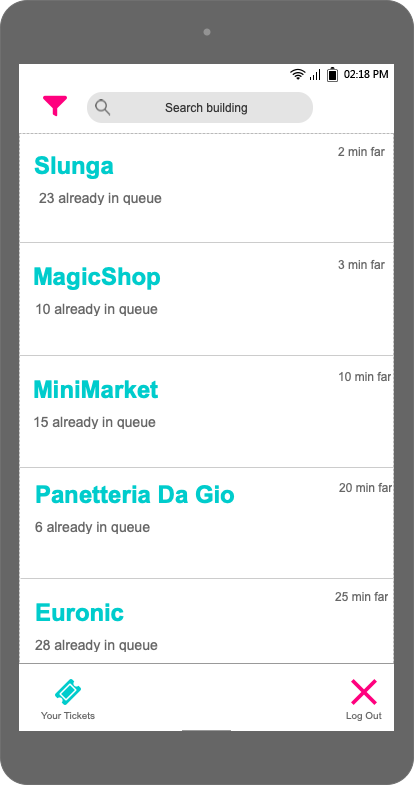
\includegraphics[width=0.33\textwidth]{/MockUps/ListOfBuildings}
	\caption{List of available buildings}
\end{figure}

\newpage

\begin{figure}[H]
	\centering
	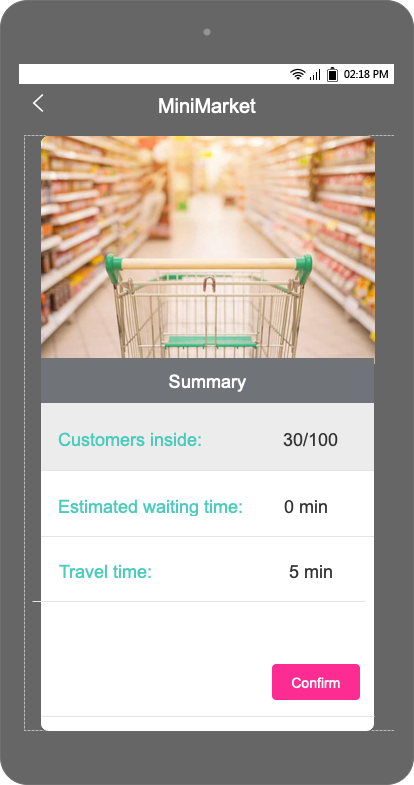
\includegraphics[width=0.33\textwidth]{/MockUps/LineUpBuilding}
	\caption{Summary page after the choice of a building to line up for.}
\end{figure}

\begin{figure}[H]
	\centering
	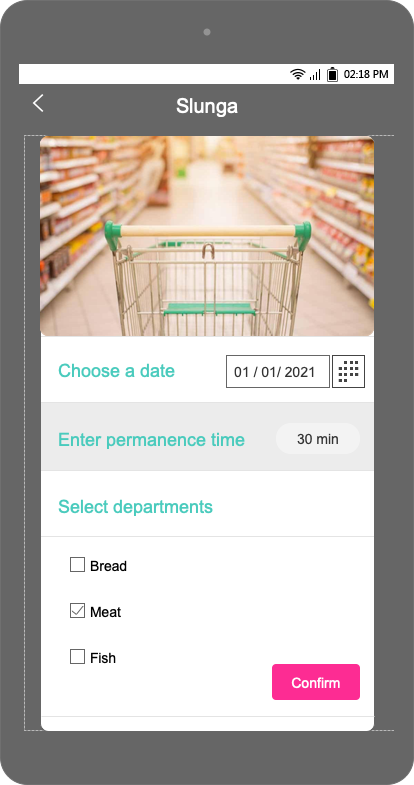
\includegraphics[width=0.33\textwidth]{/MockUps/BookingOptions}
	\caption{Options to set in order to book a time slot for the chosen building}
\end{figure}

\newpage

\begin{figure}[H]
	\centering
	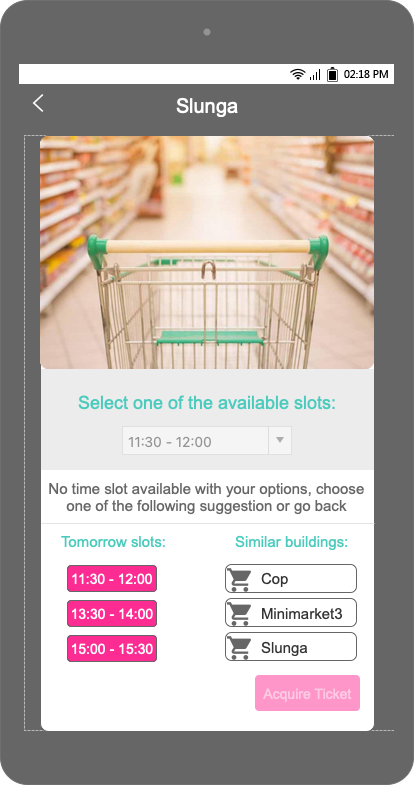
\includegraphics[width=0.33\textwidth]{/MockUps/BookingSuggestions}
	\caption{Interface to decide one of the available time slot/see alternative suggestions}
\end{figure}

\begin{figure}[H]
	\centering
	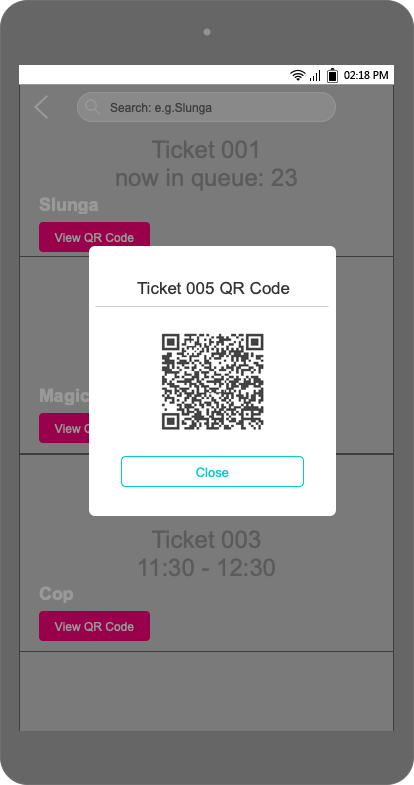
\includegraphics[width=0.33\textwidth]{/MockUps/TicketsList}
	\caption{List of tickets of a customers, with the possibility to view the related QR code}
\end{figure}
\newpage


%------------------------------------------------------------------------------------------------------------------------------------------------
\clearpage
{\color{Cerulean}{\section{Requirements Traceability}}}
\label{sect:requirements}
%Specific Requirements
	\subsection {External Interface Requirements}
	Here we provide a mapping of RASD document requirements with the Component provided in the architectural design section. The components are numerated as follows:
	\renewcommand{\theenumi}{[C\,\arabic{enumi}]}
	\begin{enumerate}
	\item TicketManager
	\item AuthManager
	\item BuildingManager
	\item GoogleMapsService
	\item DataManager
	\item MapsServiceMobileAdapter
	\item Dispatcher
	\item MapsServiceServerAdapter
	\item DBMS Service
	\item GPS Service
	\item Mobile Application
	\item Web Application
	\end{enumerate}
*GPS is an optional service, which can be or not exploited by the MobileApp user.
\newpage

\begin{table}[H]
\centering
\begin{tabular}{|c|c|c|c|c|c|c|c|c|c|c|c|c|c|} 
\hline
\rowcolor[rgb]{0.71,0.102,0} -     & C1 & C2 & C3 & C4 & C5 & C6 & C7 & C8 & C9 & C10* & C11 & C12  \\ 
\hline
{\cellcolor[rgb]{0.71,0.102,0}}R1  &    &    &    &    &    &    &    &    &    &      &     & X    \\ 
\hline
{\cellcolor[rgb]{0.71,0.102,0}}R2  &    & X  &    &    &    &    & X  &    &    &      &     & X    \\ 
\hline
{\cellcolor[rgb]{0.71,0.102,0}}R3  &    & X  &    &    &    &    & X  &    &    &      &     & X    \\ 
\hline
{\cellcolor[rgb]{0.71,0.102,0}}R4  &    & X  &    &    & X  &    & X  &    & X  &      &     & X    \\ 
\hline
{\cellcolor[rgb]{0.71,0.102,0}}R5  &    &    & X  &    &    &    & X  &    &    &      &     & X    \\ 
\hline
{\cellcolor[rgb]{0.71,0.102,0}}R6  &    &    & X  &    &    &    & X  &    &    &      &     & X    \\ 
\hline
{\cellcolor[rgb]{0.71,0.102,0}}R7  &    &    & X  &    & X  &    &    &    & X  &      &     &      \\ 
\hline
{\cellcolor[rgb]{0.71,0.102,0}}R8  &    &    & X  &    &    &    & X  &    &    &      &     & X    \\ 
\hline
{\cellcolor[rgb]{0.71,0.102,0}}R9  &    &    & X  &    & X  &    &    &    & X  &      &     &      \\ 
\hline
{\cellcolor[rgb]{0.71,0.102,0}}R10 &    & X  &    &    & X  &    & X  &    & X  &      & X   &      \\ 
\hline
{\cellcolor[rgb]{0.71,0.102,0}}R11 &    & X  &    &    & X  &    &    &    & X  &      &     &      \\ 
\hline
{\cellcolor[rgb]{0.71,0.102,0}}R12 &    & X  &    &    &    &    & X  &    &    &      & X   &      \\ 
\hline
{\cellcolor[rgb]{0.71,0.102,0}}R13 &    &    &    &    &    &    &    &    &    &      & X   &      \\ 
\hline
{\cellcolor[rgb]{0.71,0.102,0}}R14 &    & X  &    &    &    &    & X  &    &    &      & X   &      \\ 
\hline
{\cellcolor[rgb]{0.71,0.102,0}}R15 &    & X  &    &    & X  &    &    &    & X  &      &     &      \\ 
\hline
{\cellcolor[rgb]{0.71,0.102,0}}R16 &    & X  &    &    & X  &    &    &    &    &      &     &      \\ 
\hline
{\cellcolor[rgb]{0.71,0.102,0}}R17 &    & X  &    &    &    &    & X  &    &    &      & X   &      \\ 
\hline
{\cellcolor[rgb]{0.71,0.102,0}}R18 &    &    & X  & X  &    &    & X  & X  &    &      & X   &      \\ 
\hline
{\cellcolor[rgb]{0.71,0.102,0}}R19 &    &    & X  & X  & X  &    &    & X  & X  &      & X   &      \\ 
\hline
{\cellcolor[rgb]{0.71,0.102,0}}R20 &    &    & X  &    &    &    & X  &    &    & X    & X   &      \\ 
\hline
{\cellcolor[rgb]{0.71,0.102,0}}R21 &    &    & X  &    &    &    & X  &    &    &      & X   &      \\ 
\hline
{\cellcolor[rgb]{0.71,0.102,0}}R22 &    &    & X  &    &    &    & X  &    &    &      & X   &      \\ 
\hline
{\cellcolor[rgb]{0.71,0.102,0}}R23 &    &    & X  &    & X  &    & X  &    & X  &      & X   &      \\ 
\hline
{\cellcolor[rgb]{0.71,0.102,0}}R24 &    &    & X  &    & X  &    & X  &    & X  &      & X   &      \\ 
\hline
{\cellcolor[rgb]{0.71,0.102,0}}R25 &    & X  & X  &    & X  &    & X  &    & X  &      & X   &      \\ 
\hline
{\cellcolor[rgb]{0.71,0.102,0}}R26 &    & X  & X  &    & X  &    & X  &    & X  &      & X   &      \\ 
\hline
{\cellcolor[rgb]{0.71,0.102,0}}R27 &    &    & X  & X  & X  &    & X  & X  & X  &      & X   &      \\ 
\hline
{\cellcolor[rgb]{0.71,0.102,0}}R28 &    &    &    & X  &    & X  &    &    &    & X    & X   &      \\ 
\hline
{\cellcolor[rgb]{0.71,0.102,0}}R30 &    &    & X  &    & X  &    & X  &    & X  &      & X   &      \\ 
\hline
{\cellcolor[rgb]{0.71,0.102,0}}R31 &    &    &    & X  &    & X  &    &    &    & X    & X   &      \\ 
\hline
{\cellcolor[rgb]{0.71,0.102,0}}R32 & X  & X  & X  & X  &    & X  &    &    &    & X    & X   &      \\ 
\hline
{\cellcolor[rgb]{0.71,0.102,0}}R33 &    &    &    & X  &    & X  &    &    &    &      & X   &      \\ 
\hline
{\cellcolor[rgb]{0.71,0.102,0}}R35 &    &    & X  &    & X  &    &    &    & X  &      &     &      \\ 
\hline
{\cellcolor[rgb]{0.71,0.102,0}}R36 & X  & X  &    &    &    &    & X  &    &    &      & X   &      \\
\hline
\end{tabular}
\end{table}
\newpage

\begin{table}[H]
\centering
\begin{tabular}{|c|c|c|c|c|c|c|c|c|c|c|c|c|c|} 
\hline
\rowcolor[rgb]{0.71,0.102,0} -     & C1 & C2 & C3 & C4 & C5 & C6 & C7 & C8 & C9 & C10* & C11 & C12  \\ 
\hline
{\cellcolor[rgb]{0.71,0.102,0}}R37 & X  & X  &    &    &    &    & X  &    &    &      & X   &      \\ 
\hline
{\cellcolor[rgb]{0.71,0.102,0}}R38 & X  &    &    &    &    &    & X  &    &    &      & X   &      \\ 
\hline
{\cellcolor[rgb]{0.71,0.102,0}}R39 & X  &    &    &    &    &    & X  &    &    &      & X   &      \\ 
\hline
{\cellcolor[rgb]{0.71,0.102,0}}R40 & X  &    &    &    &    &    & X  &    &    &      & X   &      \\ 
\hline
{\cellcolor[rgb]{0.71,0.102,0}}R41 & X  &    & X  &    & X  &    &    &    & X  &      &     &      \\ 
\hline
{\cellcolor[rgb]{0.71,0.102,0}}R42 & X  &    &    &    &    &    & X  &    &    &      & X   &      \\ 
\hline
{\cellcolor[rgb]{0.71,0.102,0}}R43 & X  &    &    &    &    &    & X  &    &    &      & X   &      \\ 
\hline
{\cellcolor[rgb]{0.71,0.102,0}}R44 & X  &    &    &    &    &    & X  &    &    &      & X   &      \\ 
\hline
{\cellcolor[rgb]{0.71,0.102,0}}R45 &    &    & X  &    &    &    & X  &    &    &      & X   &      \\ 
\hline
{\cellcolor[rgb]{0.71,0.102,0}}R47 & X  &    &    &    &    &    & X  &    &    &      & X   &      \\ 
\hline
{\cellcolor[rgb]{0.71,0.102,0}}R48 &    &    & X  &    &    &    & X  &    &    &      & X   &      \\ 
\hline
{\cellcolor[rgb]{0.71,0.102,0}}R49 &    &    & X  &    & X  &    & X  &    & X  &      & X   &      \\ 
\hline
{\cellcolor[rgb]{0.71,0.102,0}}R50 & X  &    & X  &    & X  &    & X  &    & X  &      & X   &      \\ 
\hline
{\cellcolor[rgb]{0.71,0.102,0}}R51 & X  &    & X  &    &    &    & X  &    & X  &      & X   &      \\ 
\hline
{\cellcolor[rgb]{0.71,0.102,0}}R52 &    &    & X  &    & X  &    & X  &    & X  &      & X   &      \\ 
\hline
{\cellcolor[rgb]{0.71,0.102,0}}R53 &    &    & X  &    & X  &    & X  &    &    &      & X   &      \\ 
\hline
{\cellcolor[rgb]{0.71,0.102,0}}R54 & X  &    &    &    & X  &    & X  &    & X  &      & X   &      \\ 
\hline
{\cellcolor[rgb]{0.71,0.102,0}}R55 & X  &    &    &    & X  &    & X  &    & X  &      & X   &      \\ 
\hline
{\cellcolor[rgb]{0.71,0.102,0}}R56 & X  &    &    &    & X  &    & X  &    & X  &      & X   &      \\ 
\hline
{\cellcolor[rgb]{0.71,0.102,0}}R57 & X  & X  &    &    & X  &    & X  &    & X  &      & X   &      \\ 
\hline
{\cellcolor[rgb]{0.71,0.102,0}}R58 & X  &    &    &    &    &    &    &    &    &      &     &      \\ 
\hline
{\cellcolor[rgb]{0.71,0.102,0}}R59 & X  &    &    &    &    &    & X  &    &    &      & X   &      \\ 
\hline
{\cellcolor[rgb]{0.71,0.102,0}}R60 & X  & X  &    &    & X  &    & X  &    & X  &      & X   &      \\ 
\hline
{\cellcolor[rgb]{0.71,0.102,0}}R61 & X  & X  &    &    & X  &    & X  &    & X  &      & X   &      \\ 
\hline
{\cellcolor[rgb]{0.71,0.102,0}}R62 & X  & X  &    &    & X  &    & X  &    & X  &      & X   &      \\ 
\hline
{\cellcolor[rgb]{0.71,0.102,0}}R63 & X  &    &    &    & X  &    &    &    & X  &      &     &      \\ 
\hline
{\cellcolor[rgb]{0.71,0.102,0}}R64 & X  &    &    &    & X  &    & X  &    & X  &      & X   &      \\ 
\hline
{\cellcolor[rgb]{0.71,0.102,0}}R65 & X  &    &    &    & X  &    & X  &    & X  &      & X   &      \\ 
\hline
{\cellcolor[rgb]{0.71,0.102,0}}R66 & X  &    &    &    & X  &    & X  &    & X  &      & X   &      \\ 
\hline
{\cellcolor[rgb]{0.71,0.102,0}}R68 & X  & X  &    &    & X  &    & X  &    & X  &      & X   &      \\ 
\hline
{\cellcolor[rgb]{0.71,0.102,0}}R69 & X  & X  &    &    & X  &    & X  &    & X  &      & X   &      \\ 
\hline
{\cellcolor[rgb]{0.71,0.102,0}}R70 & X  & X  &    &    & X  &    & X  &    & X  &      & X   &      \\ 
\hline
{\cellcolor[rgb]{0.71,0.102,0}}R71 & X  &    &    &    & X  &    & X  &    & X  &      & X   &      \\ 
\hline
{\cellcolor[rgb]{0.71,0.102,0}}R72 &    & X  &    &    & X  &    & X  &    & X  &      & X   &      \\ 
\hline
{\cellcolor[rgb]{0.71,0.102,0}}R73 &    &    & X  &    & X  &    & X  &    & X  &      & X   &      \\ 
\hline
{\cellcolor[rgb]{0.71,0.102,0}}R74 & X  &    &    &    & X  &    & X  &    & X  &      & X   &      \\ 
\hline
{\cellcolor[rgb]{0.71,0.102,0}}R76 & X  &    &    &    & X  &    & X  &    & X  &      & X   &      \\ 
\hline
{\cellcolor[rgb]{0.71,0.102,0}}R77 & X  &    &    &    & X  &    & X  &    & X  &      & X   &      \\ 
\hline
{\cellcolor[rgb]{0.71,0.102,0}}R78 &    &    &    &    &    &    &    &    &    &      & X   &      \\
\hline
\end{tabular}
\end{table}
{\small R29, R34, R67, R75 are not present in the table since they have been duplicated/skipped in the RASD.}

%------------------------------------------------------------------------------------------------------------------------------------------------
\clearpage
{\color{Cerulean}{\section{Implementation, Integration and Test Plan}}}
\label{sect:implementation}
\subsection{Implementation}
\subsection{Integration}
\subsection{Test plan}


%------------------------------------------------------------------------------------------------------------------------------------------------
\clearpage
{\color{Cerulean}{\section{Effort Spent}}}
\label{sect:effort}
\begin{table}[H]
\begin{tabular}{|l|l|l|l|}
\hline
\textit{\textbf{Task}} & \textit{\textbf{Name}}        & \textit{\textbf{Time spent}}                                                                                                                                                                                                                                                                   \\ \hline
x & Francesco Attorre             & h
\\ \hline
x & Thomas Jean Bernard Bonenfant & h  
\\ \hline                                                                                                                                                                                                                                                                                     
x & Veronica Cardigliano          & h                                                                                                                                                                                                                                                                                \\ \hline
x              & Francesco Attorre             & h                                                                                                                                                                                                                                                                                 \\ \hline
x             & Veronica Cardigliano          & h                                                                                                                                                                                                                                                                                    \\ \hline
x               & Veronica Cardigliano          & h                                                                                                                                                                                                                                                                           \\ \hline
x                & Francesco Attorre             & h                                                                                                                                                                                                                                                                                \\ \hline
x                & Thomas Jean Bernard Bonenfant & h                                                                                                                                                                                                                                                                               \\ \hline
x                 & Veronica Cardigliano          & h                                                                                                                                                                                                                                                                                     \\ \hline

x              & Veronica Cardigliano          & h                                                                                                                                                                                                                                                                           \\ \hline
x              & Thoma Jean Bernard Bonenfant  & h                                                                                                                                                                                                                                                                                                                                                                                                                                                                                                                                                 \\ \hline
\end{tabular}
\end{table}

{\small comments}

%------------------------------------------------------------------------------------------------------------------------------------------------
\clearpage
{\color{Cerulean}{\section{Used Tools}}}
\color{Black}
Tools used to create this RASD document:\\
\begin {itemize}
	\item StarUML: for all the UML diagrams
	\item LaTeX: to create the pdf
	\item GitHub: for the repo of the project
	\item GoogleDoc: for a shared editing of the document
\end {itemize}

%------------------------------------------------------------------------------------------------------------------------------------------------




\end{document}